\documentclass[12pt,a4paper]{article}

\usepackage[left=20mm, right=20mm, top=20mm]{geometry} % to set up page formatting
\usepackage[skip=10pt]{parskip} % spacing in between paragraphs
\usepackage{graphicx} % Required for inserting images
\usepackage{amsmath} % Required for flexibility in mathematical equations
\usepackage{amssymb} % Required for certain math symbols e.g. E[.]
\usepackage{natbib} % Required for bibliography and citations
\usepackage{enumitem} % Required to remove gap between items in list
\usepackage{tikz} % Required to build tikz diagrams
\usepackage{xcolor} % to access colors in tikz diags
\usepackage{hyperref} % for web links
\usepackage{algorithm} % for algorithms
\usepackage{algpseudocode} % for algorithmics

\title{Discrete-event simulation model of homeless care system}
\author{Graham Burgess}
\date{\today}

\begin{document}
%
\maketitle
%
Discrete-event simulation (DES) is a form of stochastic simulation which models the evolution of a complex system according to a chronological event list which is updated throughout the simulation. DES is a powerful modeling tool given its ability to incorporate bespoke system complexities. It also naturally accomodates stochasticity by using a stream of $\text{Uniform}(\text{min} = 0, \text{max} = 1)$ pseudo-random numbers to drive the generation of random variates for model variables such as inter-arrival and service times. A single run of a DES model can be computationally cheap to run. However, one must run a DES model many times to obtain an output distribution, which means using such a model is computationally expensive.

We have developed a DES model for homeless care systems, which is based upon the DES model of \cite{singham2023discrete} for the homeless care system in Alameda County, California, US. In our model, shelter acts as a server, giving rise to a tandem queueing system, as illustrated in Figure \ref{fig:des-q}.
%
\tikzstyle{server_s} = [rectangle, rounded corners, minimum width=0.5cm, minimum height=1cm,text centered, draw=black, fill=gray!30]
\tikzstyle{server_h} = [rectangle, rounded corners, minimum width=0.5cm, minimum height=1cm,text centered, draw=black, fill=teal!30]
\tikzstyle{arrow} = [thick,->,>=stealth]
\tikzstyle{empty} = [rectangle, draw=none, fill=none]
%
\begin{figure}[h!]
  \begin{center}
    \begin{tikzpicture}
      \node (start) [empty, align=center] {};
      \node (shelter) [server_s, right of=start, xshift=3cm] {Shelter};
      \node (housing) [server_h, right of=shelter, xshift=3cm] {Housing};
      \node (end) [empty, right of=housing, xshift=1.4cm, align=center] {};
      \draw [arrow] (start) -- node [above] {Unsheltered} (shelter);
      \draw [arrow] (shelter) -- node [above] {Zero buffer}(housing);
      \draw [arrow] (housing) -- node [above] {}(end);
      \draw [arrow] (housing) to [out=265,in=195] node [below] {Partial re-entry}(shelter);
    \end{tikzpicture}
    \caption{Tandem queueing system with re-entries} \label{fig:des-q}
  \end{center}
\end{figure}
%

Here we list some key model inputs for the DES model:
%
\begin{itemize} [noitemsep]
\item Possion arrival process with rate $1$ person per day.
\item The service time at shelter is modelled as exponential with mean $6$ months.
\item The service time at housing is modelled as exponential with mean $5$ years.
\item $17\%$ of those leaving housing re-enter the queue for shelter, reflecting estimates from Alameda County.
\item Number of houses rises from $40$ to $80$ by the end of year $1$, then remains constant.
\item Number of shelters rises from $15$ to $20$ by the end of year $1$, then remains constant.
\end{itemize}
%
In Figure \ref{fig:ut-illustrative} we plot model outputs given $100$ simulation replications. 
\begin{figure}[h!]%[ut-illustrative]
    \centering
    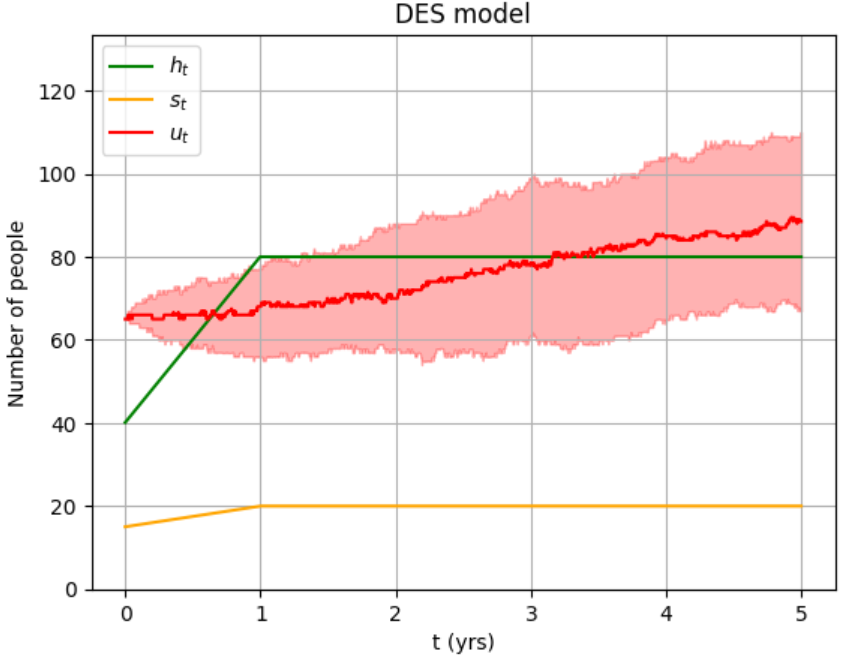
\includegraphics[scale=0.45]{example_output.png}
    \caption{DES modelling of homeless care system. Dynamics of $u_t$ (unsheltered queue) in red. Thick line shows median, with $10$th to $90$th percentile shaded. Model inputs for $s_t$ (number of shelters) and $h_t$ (number of houses) given in orange and green, respectively.}
    \label{fig:ut-illustrative}
\end{figure}
%
\bibliographystyle{apalike}
\bibliography{bibliography.bib}

\end{document}
